\chapter{Introduction}
\label{ch:introduction}

\section{Context and Motivation}
\label{sec:1.1}

The \ac{DNS}, specified by Mockapetris~\cite{RFC1034,RFC1035}, is the distributed directory service that translates domain names into \ac{IP} addresses and supports virtually every networked application on the Internet. Despite this criticality — illustrated by the Facebook \ac{DNS} outage of October 2021, which made the domain globally unresolvable for nearly six hours~\cite{Xu2023} — the \ac{DNS} has historically received less systematic measurement attention than other infrastructure layers. The most comprehensive longitudinal \ac{DNS} measurement system, OpenINTEL~\cite{vanRijswijk2016}, measures over 50\% of the global \ac{DNS} namespace daily but does so from a single vantage point in the Netherlands, leaving the geographic dimension of \ac{DNS} responses entirely uncharacterised.

\ac{DNS} data is also fundamentally ephemeral: every \ac{RR} carries a \ac{TTL} after which it is discarded~\cite{RFC1034,RFC1035}. Zone administrators can change records at any time, and the \ac{DNS} infrastructure retains no trace of previous configurations. This ephemerality motivates longitudinal archival: security researchers need historical \ac{DNS} data to reconstruct the evolution of malicious infrastructure~\cite{vanderToorn2018}; network measurement researchers need longitudinal,
geographically distributed data to characterise anycast routing and \ac{CDN} behaviour~\cite{Bortzmeyer2013,Hours2016}; infrastructure analysts need longitudinal datasets to track provider migrations and \ac{DNSSEC} deployment trends~\cite{vanRijswijk2016}.

Beyond the temporal dimension, \ac{DNS} responses exhibit a geographic dimension that single-vantage point measurement cannot observe. Three mechanisms produce this variation: (1) \textbf{\ac{CDN}-based routing} — authoritative servers return different \ac{IP} addresses depending on the inferred location of the querying resolver, directing clients to the nearest edge cluster~\cite{Li2025,Hours2016}; (2) \textbf{\ac{IP} anycast} — the same global \ac{IP} address is announced from multiple geographically distributed \ac{PoPs}, so queries from different regions reach different physical instances~\cite{Bortzmeyer2013,Koch2021}; and (3) \textbf{\ac{ECS}}~\cite{RFC7871} — the resolver embeds a truncated client \ac{IP} prefix in the query, enabling the \ac{CDN} to route by end-client location rather than resolver location~\cite{Wang2018}. 

The proportion of popular domains that return geographically differentiated responses, the magnitude and temporal stability of that differentiation, and the mechanisms that drive it remain empirically uncharacterised at population scale. This is the research gap this thesis addresses.

\bigskip
\section{DNS Resolution: a Brief Overview}
\label{sec:1.2}

Every time a browser contacts a website, a short chain of queries unfolds before any data is exchanged. \ac{DNS} handles the translation from human-readable names to numeric \ac{IP} addresses, through a hierarchy of servers distributed across the globe.

The namespace is divided into zones — administrative units, each delegated to one or more authoritative name servers that hold the canonical records for that portion of the tree. These records (\ac{RR}s) come in typed forms: an \ac{A} record binds a name to an \ac{IPv4} address; each record also carries a \ac{TTL}, after which any cached copy is considered expired.

In practice, a client application never contacts an authoritative server directly. The query goes first to the operating system's stub resolver, which forwards it to a recursive resolver — the \ac{ISP}'s, or a public alternative such as Google (8.8.8.8) or Cloudflare (1.1.1.1). If the recursive resolver holds a valid cached answer, it returns it immediately. If not, it iterates down the hierarchy — from the root servers through the appropriate \ac{TLD} server, down to the domain's own authoritative servers — retrieves the answer, caches it for the \ac{TTL} duration, and passes it back to the client. Figure~\ref{fig:DNS_resolution} illustrates this process.

\begin{figure}[tp]
  \centering
  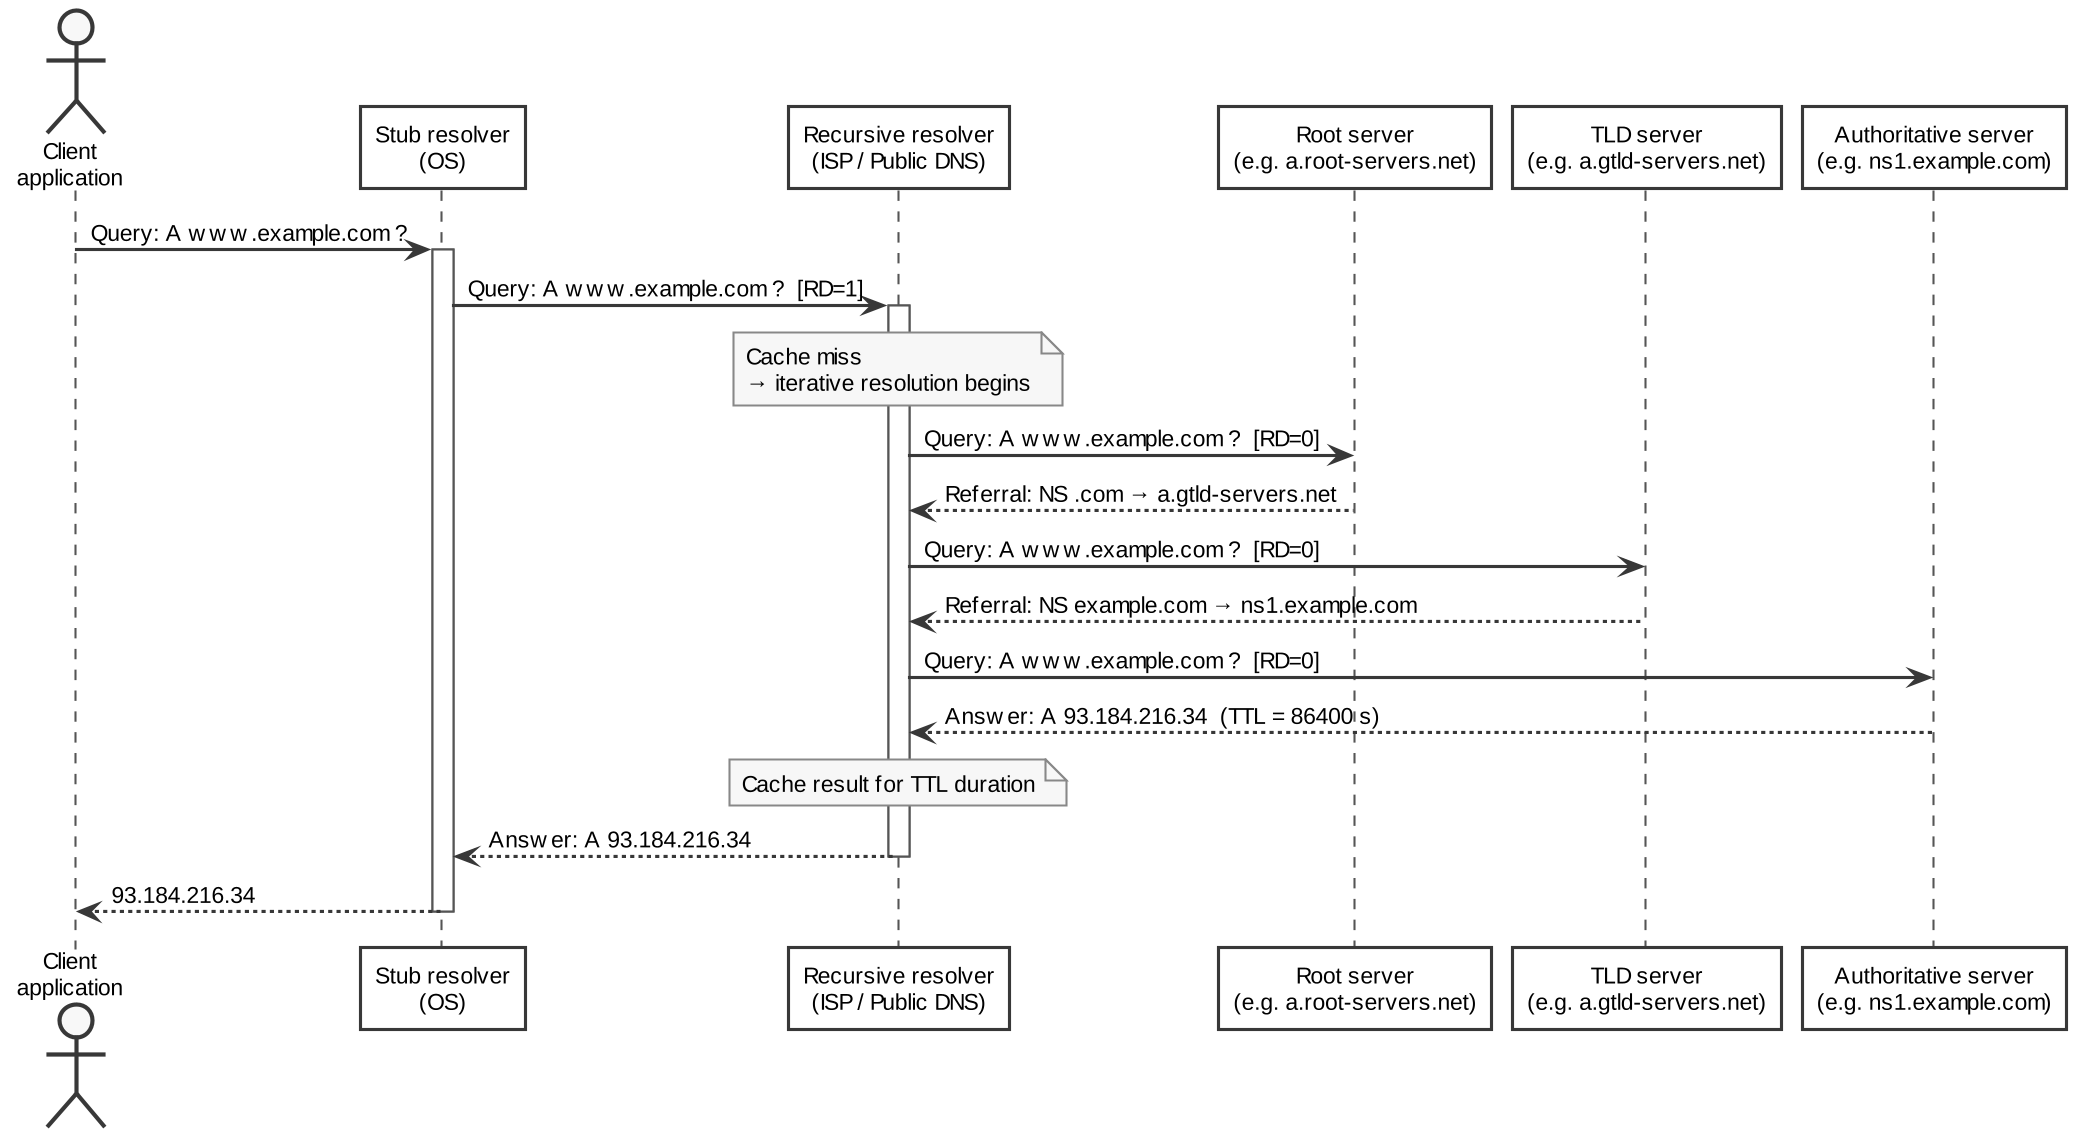
\includegraphics[width=0.92\linewidth]{figures/fig1_dns_resolution.png}
  \caption{Iterative \ac{DNS} resolution process. The client-side resolver (stub) forwards the query to a recursive resolver, which performs three successive referral queries (root $\rightarrow$ \ac{TLD} $\rightarrow$ authoritative) before returning the final answer. The \ac{TTL} field in the authoritative response governs how long the recursive resolver caches the result.}
  \label{fig:DNS_resolution}
\end{figure}

This architecture has two consequences central to this thesis. First, the recursive resolver acts as a geographic proxy: from the authoritative server's perspective, all queries originating from the same recursive resolver appear to come from a single location, regardless of where the end-users actually are. \ac{CDN} operators exploit this to tailor answers by resolver location. Second, because any resolver can query any authoritative server, it is possible to measure how authoritative servers respond to queries from different geographic vantage points — which is precisely the approach taken in Chapter~\ref{ch:method}.

\bigskip
\section{Research Questions and Objectives}
\label{sec:1.3}

This thesis addresses the following main research question:

\textit{How can one design and deploy a distributed \ac{DNS} measurement system that captures the geographic and temporal diversity of \ac{DNS} responses for the most popular domains on the web, in a manner that is ethically sound, reproducible, and useful to the research community?}

Four operational sub-questions guide the empirical analysis:

\textbf{Q1 — Geographic diversity}: What proportion of popular domains return different \ac{DNS} responses depending on query origin, and which mechanisms (\ac{CDN} routing, anycast, \ac{ECS}) explain the differentiation? 

Measuring the full Tranco Top-10K would require on the order of 10,000 concurrent RIPE Atlas measurements, far exceeding typical account limits; this thesis therefore focuses on the Tranco Top-250, which concentrates on the highest-traffic domains where geographic differentiation is most prevalent and the findings most practically relevant.


\textbf{Q2 — Temporal stability}: What is the temporal stability of \ac{DNS} responses at day, week, and month timescales over the measurement period?

\textbf{Q3 — RIPE Atlas geographic bias}: Do the documented geographic biases of the RIPE Atlas probe distribution~\cite{Bajpai2017} (91\% of probes in Europe/North America) significantly affect the ability to observe \ac{DNS} geographic variation?

\textbf{Q4 — Resolver impact}: Do the three major public \ac{DNS} resolvers (Google 8.8.8.8, Cloudflare 1.1.1.1, Quad9 9.9.9.9) return consistent \ac{DNS} responses for the same domain queried from the same geographic location, and how large is the inter-resolver divergence?

To answer these questions, the thesis designs, implements, and operates a measurement system that: (1) measures the Tranco Top 250 domains~\cite{LePochat2019} daily over 50 days — a duration chosen to cover at least one complete monthly cycle, enabling analysis of \ac{DNS} stability at the day, week, and month timescales required by Q2; (2) collects measurements from $\approx$200 globally distributed RIPE Atlas probes selected via RIPE Atlas geographic zone-based distribution; (3) archives results in Parquet format following \ac{FAIR} data principles; and (4) analyses the dataset to produce quantitative answers to Q1–Q4. The measurement design complies with the RIPE Atlas ethical guidelines~\cite{Kisteleki2016}: all queried domains are publicly accessible, measurement frequency respects \ac{DNS} \ac{TTL}s, and no politically sensitive content is included.

\bigskip
\section{Thesis Structure}
\label{sec:1.4}

\textbf{Chapter~\ref{ch:state-of-the-art}} reviews the state of the art across five domains: \ac{DNS} measurement paradigms and the OpenINTEL infrastructure; the RIPE Atlas platform and its biases; anycast routing and \ac{NSID}-based instance identification; \ac{CDN} \ac{DNS} routing and \ac{ECS}; and domain ranking lists, concluding with a gap analysis.

\textbf{Chapter~\ref{ch:method}} describes the full measurement methodology: Tranco corpus configuration, RIPE Atlas probe selection and stratification, \ac{DNS} measurement parameters, data collection pipeline, and Parquet storage architecture.

\textbf{Chapter~\ref{ch:results}} presents the empirical results of the measurement campaign: dataset statistics and answers
to Q1–Q4 with quantitative evidence and visualisations.

\textbf{Chapter~\ref{ch:conclusion}} discusses the results in light of the literature, evaluates study limitations, and draws
conclusions with future research directions.